\documentclass[ngerman]{article}
\usepackage{babel}
\usepackage{tikz}
\usetikzlibrary{arrows.meta}
\usepackage[screen]{geometry}

\begin{document}

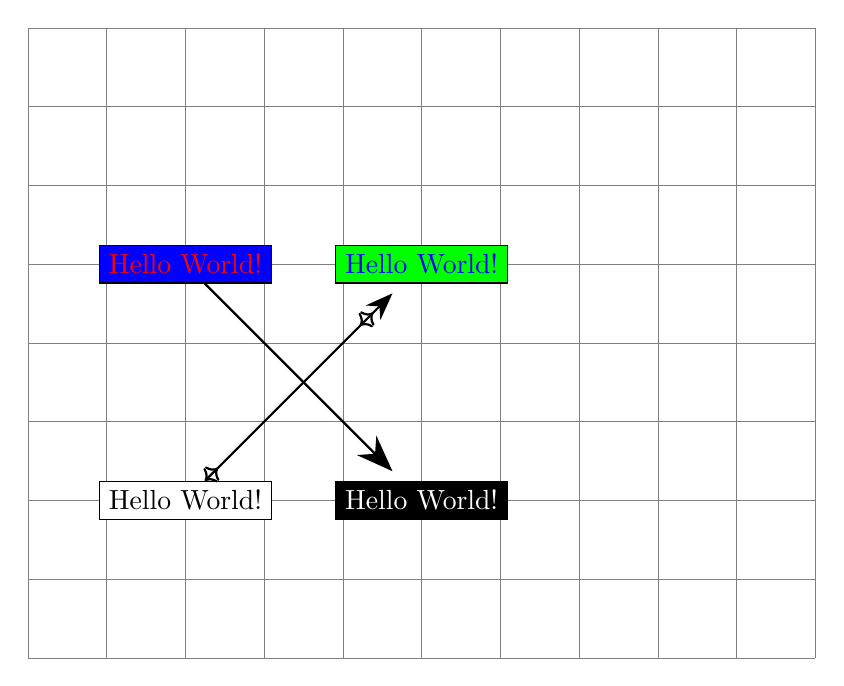
\begin{tikzpicture}[shorten >= 5pt]

    \draw[help lines](0, 0) grid (10, 8);

    \path node (a) [draw, fill=blue, text=red] at (2, 5) {Hello World!};
    \path node (b) [draw, fill=white, text=black] at (2, 2) {Hello World!};
    \path node (c) [draw, fill=black, text=white] at (5, 2) {Hello World!};
    \path node (d) [draw, fill=green, text=blue] at (5, 5) {Hello World!};

    \draw[->, thick,arrows={-Stealth[scale=2]}] (a) -- (c);
    \draw[->, thick,arrows={<>-<>Stealth[scale=1.5]}] (b) -- (d);

\end{tikzpicture}

\end{document}

